\section*{5. Field-Programmable Gate Array}
\addcontentsline{toc}{chapter}{Field-Programmable Gate Array}

A field-programmable gate array (FPGA) is an integrated circuit designed to be configured by a customer or a designer after manufacturing – hence the term "field-programmable". The FPGA configuration is generally specified using a hardware description language (HDL), similar to that used for an application-specific integrated circuit (ASIC). Circuit diagrams were previously used to specify the configuration, but this is increasingly rare due to the advent of electronic design automation tools.\vspace{.3cm}

FPGAs contain an array of programmable logic blocks, and a hierarchy of "reconfigurable interconnects" allowing blocks to be "wired together", like many logic gates that can be inter-wired in different configurations. Logic blocks can be configured to perform complex combinational functions, or merely simple logic gates like AND and XOR. In most FPGAs, logic blocks also include memory elements, which may be simple flip-flops or more complete blocks of memory. Many FPGAs can be reprogrammed to implement different logic functions, allowing flexible reconfigurable computing as performed in computer software. FPGAs have a remarkable role in embedded system development due to their capability to start system software (SW) development simultaneously with hardware (HW), enable system performance simulations at a very early phase of the development, and allow various system partitioning (SW and HW) trials and iterations before final freezing of the system architecture.\vspace{.3cm}

\begin{figure}[h]
	\centering
	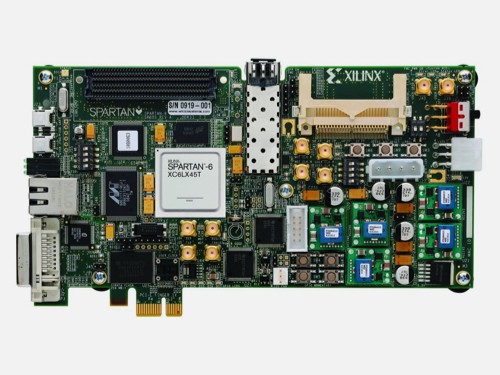
\includegraphics[width=0.7\linewidth]{images/1586365527662}
	\captionsetup{labelformat=empty}
	\caption{Field-Programmable Gate Array}
\end{figure}


\subsection*{5.1 History}
The FPGA industry sprouted from programmable read-only memory (PROM) and programmable logic devices (PLDs). PROMs and PLDs both had the option of being programmed in batches in a factory or in the field (field-programmable). However, programmable logic was hard-wired between logic gates.\vspace{.3cm}

Altera was founded in 1983 and delivered the industry's first reprogrammable logic device in 1984 – the EP300 – which featured a quartz window in the package that allowed users to shine an ultra-violet lamp on the die to erase the EPROM cells that held the device configuration.\vspace{.3cm}

Xilinx co-founders Ross Freeman and Bernard Vonderschmitt invented the first commercially viable field-programmable gate array in 1985 – the XC2064. The XC2064 had programmable gates and programmable interconnects between gates, the beginnings of a new technology and market. The XC2064 had 64 configurable logic blocks (CLBs), with two three-input lookup tables (LUTs). More than 20 years later, Freeman was entered into the National Inventors Hall of Fame for his invention.\vspace{.3cm}

In 1987, the Naval Surface Warfare Center funded an experiment proposed by Steve Casselman to develop a computer that would implement 600,000 reprogrammable gates. Casselman was successful and a patent related to the system was issued in 1992.\vspace{.3cm}

Altera and Xilinx continued unchallenged and quickly grew from 1985 to the mid-1990s when competitors sprouted up, eroding a significant portion of their market share. By 1993, Actel (now Microsemi) was serving about 18 percent of the market. By 2013, Altera (31 percent), Actel (10 percent) and Xilinx (36 percent) together represented approximately 77 percent of the FPGA market.\vspace{.3cm}

The 1990s were a period of rapid growth for FPGAs, both in circuit sophistication and the volume of production. In the early 1990s, FPGAs were primarily used in telecommunications and networking. By the end of the decade, FPGAs found their way into consumer, automotive, and industrial applications.\vspace{.3cm}

Companies like Microsoft have started to use FPGAs to accelerate high-performance, computationally intensive systems (like the data centers that operate their Bing search engine), due to the performance per watt advantage FPGAs deliver. Microsoft began using FPGAs to accelerate Bing in 2014, and in 2018 began deploying FPGAs across other data center workloads for their Azure cloud computing platform.\vspace{.3cm}

\subsection*{5.2 Applications}
An FPGA can be used to solve any problem which is computable. This is trivially proven by the fact that FPGAs can be used to implement a soft microprocessor, such as the Xilinx MicroBlaze or Altera Nios II. Their advantage lies in that they are significantly faster for some applications because of their parallel nature and optimality in terms of the number of gates used for certain processes.\vspace{.3cm}

FPGAs originally began as competitors to CPLDs to implement glue logic for printed circuit boards. As their size, capabilities, and speed increased, FPGAs took over additional functions to the point where some are now marketed as full systems on chips (SoCs). Particularly with the introduction of dedicated multipliers into FPGA architectures in the late 1990s, applications which had traditionally been the sole reserve of digital signal processor hardware (DSPs) began to incorporate FPGAs instead.\vspace{.3cm}

Another trend in the use of FPGAs is hardware acceleration, where one can use the FPGA to accelerate certain parts of an algorithm and share part of the computation between the FPGA and a generic processor. The search engine Bing is noted for adopting FPGA acceleration for its search algorithm in 2014. As of 2018, FPGAs are seeing increased use as AI accelerators including Microsoft's so-termed "Project Catapult" and for accelerating artificial neural networks for machine learning applications.\vspace{.3cm}

Traditionally,[when?] FPGAs have been reserved for specific vertical applications where the volume of production is small. For these low-volume applications, the premium that companies pay in hardware cost per unit for a programmable chip is more affordable than the development resources spent on creating an ASIC. As of 2017, new cost and performance dynamics have broadened the range of viable applications.\vspace{.3cm}

The company Gigabyte created an i-RAM card which used a Xilinx FPGA although a custom made chip would be cheaper if made in large quantities. The FPGA was chosen to bring it quickly to market and the initial run was only to be 1000 units making an FPGA the best choice. This device allows people to use computer ram as a hard drive.\vspace{.3cm}